\documentclass[a4paper,12pt,oneside,brazil,english,nottoc,notbib]{abntex2}

% =============================
% ==== BIBLIOTECAS ====
% =============================
\usepackage{lmodern} % Mudar fonte padrão
\usepackage[T1]{fontenc}
\usepackage[utf8]{inputenc}
\usepackage{babel}
\usepackage{geometry}
\usepackage{ragged2e}
\usepackage{graphicx}
\usepackage{xcolor}
\usepackage{amsmath}
\usepackage{titlesec}
\usepackage{etoolbox}
\usepackage{tocloft}
\usepackage[alf,abnt-etal-list=2,abnt-etal-cite=1,abnt-doi=link,abnt-url-package=hyperref,abnt-emphasize=bf]{abntex2cite}
% Tabelas
\usepackage{tabularx}
\usepackage{adjustbox}
\usepackage{booktabs}

% ==== Sumario com seções principais em negrito ====
\renewcommand{\ABNTEXsectionfont}{\bfseries}

\usepackage{fancyhdr}
\usepackage{appendix}
\usepackage{setspace}
\usepackage{titling}
\usepackage{hyperref}
\usepackage{lipsum}
\usepackage{float}
\usepackage{caption}

% ==== Ajuste do nome para figuras ====
\addto\captionsenglish{\renewcommand{\figurename}{Graph}}

% ==== Ambiente para quadros ====
\newfloat{quadro}{htbp}{loq}
\floatname{quadro}{Quadro}

% ==== Customizacoes tocloft ====
\newcommand{\listabstractname}{Abstract}
\newcommand{\addabstracttoc}{%
  \addcontentsline{toc}{section}{\protect\numberline{}\listabstractname}%
}
\renewcommand{\cftsecindent}{1.5em}

% =============================
% ==== LAYOUT E MARGENS ====
% =============================
\geometry{top=3cm, bottom=2cm, left=3cm, right=2cm}
\setlength{\parindent}{1.25cm}
\onehalfspacing

% ==== Cabecalho e rodape ====
\setlength{\headheight}{24.63824pt}
\pagestyle{plain}
\fancyhf{}
\fancyhead[L]{\fontsize{9.5pt}{11pt}\selectfont
\includegraphics[height=1cm]{Figuras/usp_logo.png}}
\fancyhead[R]{\fontsize{9.5pt}{11pt}\selectfont\raisebox{0.25cm}{\textcolor{gray}{PhD Thesis Proposal}}}
\fancyfoot[C]{\fontsize{9.5pt}{11pt}\selectfont\textcolor{darkgray}{\textbf{\thepage}}}

% =============================
% ==== ESTILOS ====
% =============================
\titleformat{\section}{\bfseries\Large}{\thesection}{1em}{}
\titleformat{\subsection}{\bfseries\large}{\thesubsection}{1em}{}
\titleformat{\subsubsection}{\normalfont\normalsize}{\thesubsubsection}{1em}{}
\titleformat{\paragraph}{\normalfont\normalsize}{\theparagraph}{1em}{}

% ==== Numeracao com ponto ====
\renewcommand{\thesection}{\arabic{section}.}
\renewcommand{\thesubsection}{\arabic{section}.\arabic{subsection}.}
\renewcommand{\thesubsubsection}{\arabic{section}.\arabic{subsection}.\arabic{subsubsection}.}
\renewcommand{\theparagraph}{\arabic{section}.\arabic{subsection}.\arabic{subsubsection}.\arabic{paragraph}.}

% ==== Redefine secao de referencias ====
\makeatletter
\renewcommand\bibsection{%
  \clearpage
  \phantomsection
  \section*{References}%
  \addcontentsline{toc}{section}{\protect\numberline{}References}%
  \thispagestyle{fancy}%
}
\makeatother

% ==== Configuracao do hyperref ====
\hypersetup{
    colorlinks=true,
    linkcolor=black,
    citecolor=black,
    urlcolor=black,
    pdftitle={Economic Commensalism: Governing the Commons through Rational Incentives},
    pdfauthor={Fernando Souza da Vieira}
}

% =============================
% ==== INICIO DO DOCUMENTO ====
% =============================
\begin{document}

% ==== CAPA ====
\pagenumbering{roman}
\begin{titlepage}
    \centering
    {\large UNIVERSITY OF S\~AO PAULO (USP)\\[0.2cm]
    FACULTY OF ECONOMICS, ADMINISTRATION AND ACCOUNTING\\
    OF RIBEIR\~AO PRETO (FEARP)}\\[3.5cm]

    {\Huge \bfseries Economic Commensalism:}\\[0.3cm]
    {\LARGE Governing the Commons through Rational Incentives}

    \vspace{1.5cm}

    {\large \textbf{Doctoral Researcher: Fernando Souza da Vieira}}\\[0.3cm]
    {\large \textbf{Advisor: Prof. Dr. Alexandre Chibebe Nicolella}}\\[2cm]

    \textit{Research Proposal for the PhD in Applied Economics}\\
    University of S\~ao Paulo (FEARP/USP)\\[2.5cm]

\vfill
{\large Ribeir\~ao Preto, SP}\\[0.3cm]
{\large June, 2025}

\end{titlepage}

% ==== SUMARIO ====
\clearpage
\begingroup
\selectlanguage{english}
\renewcommand{\addcontentsline}[3]{}
\tableofcontents
\endgroup
\clearpage

% ==== PAGINA INICIAL ====
\pagenumbering{arabic}
\setcounter{page}{5}
\pagestyle{fancy}

% ==== ABSTRACT ====
\clearpage
\addabstracttoc
\section*{Abstract}

%%%===========================================
% \phantomsection
% \addcontentsline{toc}{section}{Abstract}

% =============================
% \section*{Abstract}
% =============================

\textbf{Environmental degradation often results from the socially burdensome trade-off between boosting productivity and overexploiting natural resources.} Two primary modes of resource use dominate this dynamic: extractivism and predation. Extractivism involves the removal of natural resources in a manner that, although potentially impactful, can ostensibly occur within regenerative or sustainable limits. By contrast, predation refers to the indiscriminate and often illegal depletion of renewable or non-renewable resources, such as through the burning of public lands or the extraction of minerals on indigenous territories, typically disregarding environmental laws and property rights.

These tensions between economic agents and environmental advocates permeate broader legal, ethical, and ecological paradigms that are difficult to stabilize socially and economically. As a result, the use of shared natural resources often evolves into a condition of imperfect competition, where productive agents, environmental organizations, and policymakers each act to optimize their interests at the expense of collective welfare.

\textbf{This research introduces an alternative perspective to reconciling environmental preservation and economic interests through the concept of \emph{economic commensalism}, which frames economic relations around rational neutrality in the use of natural resources. By repositioning private incentives to align with collective environmental goals, the framework fosters voluntary adherence to sustainable practices and aims to stabilize long-term ecological and economic outcomes through rational, market-based mechanisms.} Unlike traditional models that address environmental externalities primarily through corrective tools such as Pigouvian taxes, Coasian bargaining, Pareto efficiency, and others, or the prevailing institutional applied, based wether coercion wether sparse, inefficient, and unstructured positive incentives, this approach seeks to internalize ecological sustainability within the economic decision-making process itself.

\textbf{This thesis is structured around three complementary components:} \textbf{(i) a theoretical framework}, which employs intertemporal optimization methods, uncertainty management techniques, and dynamic learning processes to model decision-making behavior among economic agents; \textbf{(ii)} \textbf{mathematical modeling}, which formalizes the proposed mechanisms; \textbf{and (iii) empirical validation}, which tests their practical feasibility by applying these models to Brazil’s Mato Grosso region, an area marked by deforestation and agricultural expansion. \textbf{The research thus seeks to contribute to both economic theory and policy design by proposing a market-driven mechanism whereby economic actors voluntarily engage in sustainable practices while preserving economic returns and long-term viability.}

\newpage

% fim %

% ==== ORGANIZACAO DAS SECOES ====
\clearpage
\thispagestyle{fancy}

% ===
\section{Introduction}
% ===

From an efficiency perspective, neither extreme predation, marked by the indiscriminate and often illegal depletion of natural resources, nor strict mutualism, characterized by minimal or non-extractive use of the environment, leads to a Pareto-optimal equilibrium \cite{dasgupta2001human}. These two poles represent opposing boundaries of environmental interaction: the former disregards sustainability entirely, while the latter may overly constrain productive potential \cite{ostrom1990commons}. Situated between these extremes, extractivism has become the prevailing paradigm in both economic theory and practice, advocating resource use within ostensibly sustainable or regenerative limits. 

Yet even extractivism, when poorly regulated, can drift toward inefficiency: on one hand, overly restrictive preservation may inhibit activities that could enhance welfare without compromising ecological stability; on the other, unchecked exploitation produces negative externalities that degrade shared inputs vital to multiple stakeholders \cite{chichilnisky2017north}. As such, when natural resource allocation is left entirely to market forces, it tends to deviate from Pareto efficiency due to either underutilization or overuse, highlighting the need for corrective mechanisms that better align private incentives with socially optimal outcomes \cite{hanley2007environmental}.

In tandem with this, economics consistently defines the factors of production as land (N), capital (K), and labor (L), the fundamental inputs in the transformation process of goods and services. Although environmental elements are directly or indirectly embedded in all three, standard economic models have historically treated the environment as an exogenous variable, implicitly assuming its unlimited availability \cite{jehle2011}. As a result, ecological constraints are often ignored or only marginally considered through land productivity, which affects land rents based on natural attributes such as fertility, location, and regenerative capacity \cite{article}.

In response to the ongoing environmental degradation, over the past decades, a range of institutional efforts has been undertaken to curb environmental disasters such as global warming, tropical deforestation, and the indiscriminate or illegal exploitation of water and soil resources. International agreements such as the Kyoto Protocol (1997), the Paris Agreement (2015), and the Convention on Biological Diversity (1992), as well as regional initiatives and national policies, have established frameworks for emission reduction, biodiversity conservation, and sustainable resource management. Not necessarily considering human self-interest over ecological needs, these instruments often rely on legally binding commitments, emission trading systems, reforestation programs, and technological cooperation mechanisms \cite{easterly2013tyranny}.

In a related vein, legal and institutional instruments have been established to create a system of checks and balances capable of inhibiting irrational environmental exploitation in the short and medium term, while fostering ecological awareness in the long term. For example, the Brazilian Forest Code (Lei nº 12.651/2012) stands out as a key legal framework regulating land use and native vegetation preservation in rural properties within the country's borders \cite{brasil2012florestal}, while non-governmental organizations (NGOs) such as Greenpeace, the World Wide Fund for Nature (WWF), the Rainforest Foundation, Imazon (Instituto do Homem e Meio Ambiente da Amazônia), among many others, play a crucial role in monitoring compliance, raising public awareness, and pressuring both governments and corporations to adopt more sustainable practices throughout the world \cite{lomborg2001skeptical}. 

Despite their relevance, such efforts often reflect a moralistic or idealized form of environmentalism. While rhetorically aimed at fostering mutualistic relationships between humans and nature, they often result in a regulated form of extractivism. Legal frameworks such as the Forest Code impose rigid constraints that, while intended to protect native ecosystems, fail to align with the economic rationale of landowners, who often perceive them not as incentives for sustainable coexistence, but as punitive restrictions that prevent them from fully utilizing a productive factor — land — under their control \cite{agrawal2005environmentality}. This maladjustment not only generates resistance and non-compliance but also fuels a broader sense of injustice among rural producers, who feel disproportionately burdened by conservation obligations without corresponding compensatory mechanisms \cite{borner2016mixing}.

Theoretical and applied economics, in turn, has addressed environmental issues with the common understanding that markets fail to internalize ecological costs. Without some form of coercive intervention — usually by governments — such failures tend to generate vicious long-term outcomes. For instance, \citeonline{pigou2010liberty} have proposed tariffs (Pigouvians taxes) as a way to internalize negative environmental externalities alongside its neoclassical model. In his view, \citeonline{hardin1968tragedy} argued that, in the absence of private property or state regulation, individual self-interest leads to what he called the "tragedy of the commons", a situation in which natural resources are completely exhausted as a result of individuals aiming to maximize their own utility, while the common good is entirely neglected. 

Alternatively, \citeonline{ostrom2002commonpool} challenged Hardin’s dilemma by arguing that, under certain institutional conditions, the self-management of natural resources can be sustainable. \citeonline{assuncao2013deterring} highlight that enforcement, when paired with well-designed incentives, has shown results in reducing Amazon deforestation, yet faces structural and political resistance when scaled. \citeonline{scheinkman2008social}’s contributions to the modeling of local interactions and externalities provide a relevant foundation for understanding how decentralized behavior can lead to socially suboptimal equilibria, especially in resource use contexts. 

Since the mid-1980s, the so-called Green Economy has advanced the argument that economic development is only viable if improvements in human well-being are balanced with reductions in environmental risks and ecological scarcity \cite{jacobs1991green}. According to this school of thought, the economy must stop treating the environment as a substitute good and begin to value it as a complementary asset. This implies ensuring that each generation inherits an ecosystem that is at least equivalent in quality and function, recognizing that many ecological characteristics are irreplaceable. Such an approach is framed not only by the risks of irreversibility and uncertainty but also by the moral imperative of intergenerational equity \cite{pearce1989blueprint}.

As we can see, throughout history, a persistent misalignment has existed between collective supply and private demand in the use of natural resources, which leads to misconduct on the part of certain private agents who do not consider it fair to internalize diffuse social costs in individual operations, all of this intertwined in a non-standardized and inefficient institutional-legal scheme, operated by States and monitored by the third sector. Despite advances in theory and policy, a deeper problem persists: the economic system — including markets, institutions, and even economic theory — struggles to adequately conceptualize and resolve the trade-off between development and sustainability. 

Apparently, an endless back-and-forth dilemma is presented as an unsolvable tension between collective morality and individual utilitarianism. In the end, nature seems to be on a path of degradation that initially affects vulnerable regions, but eventually reaches everyone, as environmental collapse leads to widespread economic consequences such as global warming, water scarcity, and the increasing threat to agricultural and ecological food systems. This apparent antagonism may in fact be rooted in theoretical and institutional misalignments, rather than from an inherent incompatibility between individual incentives and ecological responsibility, a conjecture explored throughout this study.

% ---
\subsection{Motivations}
% ---

As demonstrated, despite their normative relevance and global reach, the implementation and effectiveness of actions taken by governments, NGOs, the media, academia, and public opinion are persistently challenged by the economic interests and political imperatives of productive agents and decision-makers. In many cases, short-term economic gains and competitive pressures continue to override long-term sustainability goals, limiting the transformative potential of these institutional frameworks.

The practical outcome of this trade-off between economics and ecology has often been the over-exploitation of natural resources, leading to negative externalities such as the depletion of land productivity, pollution of air, soil, rivers, and other water sources, disruption of hydrological cycles, increase in agricultural pests, and rising production costs. These impacts have not only degraded biomes and ecosystems but also compromised the quality of life and the productive capacity of the economic agents involved. The indiscriminate use of natural resources — treated as exogenous and not subject to scarcity analysis — has led to reactive approaches aimed at correcting the resulting instabilities, such as the overuse and declining utility of key productive inputs like land, water, and air.

Mato Grosso serves as the heart of Brazil's agricultural expansion and hosts three primary biomes: the Amazon, Cerrado, and Pantanal. It offers a compelling empirical and conceptual context for this study. The region faces escalating challenges from deforestation, rising global commodity needs, and new sustainability obligations. These factors position the state at the intersection of risks and opportunities in the move towards environmentally sustainable practices that align with economic incentives. The region's blend of significant environmental value and robust production creates a scenario to test if rational eco-economic dynamics — similar to those in the economic commensalism framework — can harmonize productivity with sustainable conservation without relying solely on coercion or moral appeals.

Typical examples of this concern, a dual perspective emerges from the land and burgeoning carbon markets, shedding light on the complexities of environmental and economic interactions. Land is still regarded as a static input within traditional production models, yet its ecological value, particularly when conserved, tends to lack proper valuation or is grossly undervalued. Likewise, carbon, although recognized as a marketable commodity in both voluntary and regulatory contexts, often fails to reflect the spatial dynamics of land utilization and ecosystem sturdiness. These discrepancies create contradictory motivations for producers, who gain incentives to enlarge their productive areas but face indirect penalties for land conservation, despite the potential for conservation to offer quantifiable ecological benefits and financial gains. This discord highlights the necessity for a novel theoretical framework that integrates the environment as a core economic element.

Given the opportunity costs faced by producers and consumers, traditional solutions — such as Pigouvian taxes, regulatory enforcement, community governance, and incentive-based schemes — have provided only partial answers. These approaches often fail to account for long-term ecological uncertainty, interdependent decision-making among producers, and the endogenous learning behaviors — involving agricultural producers, ecologists, politicians, consumers, public opinion and legal instruments — that shape conservation outcomes. This conceptual and institutional gap motivates the search for a more integrated and incentive-compatible framework, which constitutes the foundation of the present study.

% ---
\subsection{Rationale}
% ---
% Por que este problema merece ser estudado do ponto de vista conceitual, histórico ou lógico?
% Lógica interna

Despite decades of theoretical development, current approaches to environmental economics still fail to endogenize natural resources within production decisions. Orthodox models treat the environment as an exogenous factor, while corrective instruments such as taxes or command-and-control mechanisms face limitations in efficiency, grounded in assumptions such as the environment being regulatable as a nearly homogeneous entity, carbon being a universal proxy for compensation, and human rationality being static and ubiquitous. 

Thus, although significant theoretical advances and practical attempts have been made in integrating environmental concerns into economic decision-making, important shortcomings remain. Taxes, legal embargoes, property rights, and — as the following chapters will demonstrate through theoretical and empirical evidence — carbon markets have fallen short of delivering on both environmental and economic expectations. 

% ---
\subsection{Justification}
% ---

Although carbon markets, environmental certifications, regulatory constraints, and coercive enforcement mechanisms have become widespread, these tools have not been effective in changing the core economic behaviors that lead to environmental harm. Carbon credits frequently lack connection to the specific ecological settings and fail to provide incentives that are accessible, predictable, or appealing to producers. Certifications primarily advantage a limited group already aligned with sustainability ideals, while legal enforcement struggles with weak institutions, limited monitoring capabilities, and strategic circumvention. These measures often function outside the decision-making frameworks of agents, viewing the environment as a limitation rather than an opportunity. This disconnect suggests the necessity for a model where environmental preservation is embedded within agents’ rational decision-making, not as an external requirement, but as a strategic advantage, which is the foundation of the economic commensalism framework presented in this study.

These limitations reveal the need for a new paradigm capable of reconciling production incentives with environmental preservation. In this context, the concept of \textit{economic commensalism} is proposed as a stable framework through which economic agents can align individual profitability with collective ecological sustainability, provided that suitable incentive structures are in place. 

This work aims to be relevant by highlighting how economic theory can be improved, and this will not only clarify what and why current environmental preservation mechanisms do not work properly — which include the carbon market, environmental certificates and targets for controlling the use of natural resources —, but will also provide, through a stable and well-founded theoretical framework, ways to improve market instruments and state actions related to environmental preservation without necessarily compromising the economic interests of the agents involved.


\newpage

% fim %
\clearpage
\thispagestyle{fancy}
% ===
\section{Research Design}
% ===

Building on the conceptual discussion presented in the previous section, this study now outlines its research design, which integrates theoretical modeling with empirical investigation. Given the structural limitations of current environmental economic approaches, particularly their exogenous treatment of ecological variables, the research seeks to construct and test an alternative framework grounded in the principle of economic commensalism.

To that end, this section presents the research problem, hypotheses, objectives, and methodological foundations that guide the study. By combining dynamic optimization, learning models, and institutional analysis, we aim to assess whether incentive-compatible public policies can reconcile individual profitability with long-term sustainability preservation.

This thesis is organized into three principal sections to implement its objectives: two theoretical chapters and an empirical chapter. The opening chapter lays out the ontological and epistemological underpinnings of economic commensalism, introduces a typology for ecological-economic strategies, and critiques the shortcomings of traditional models. The second chapter constructs a formal dynamic model, integrating Bellman equations, elements of game theory, and learning processes, to assess the internal coherence and logical outcomes of the proposed framework. The final chapter performs an econometric and geospatial analysis using real-world data from Mato Grosso to determine if the theoretical model's predictions hold true in practice. Collectively, these components intend to offer conceptual clarity, mathematical precision, and empirical significance to the study's key assertion.

% ---
\subsection{Problem}
% ---

In light of the constraints inherent within existing economic theory and contemporary institutional and legal proposals, the \textbf{research problem} of this study is to answer the following question: 
\vspace{1em}

\begin{flushright}
\begin{minipage}{0.93\linewidth}
\noindent
\hspace{0.4em}\vrule width 0.4pt height 5.5em \hspace{1.2em}%
\parbox[b]{0.95\linewidth}{
\textit{Is it possible to effectively and efficiently reconcile private productivity and profitability with socially desirable environmental preservation through well-structured economic incentives, surpassing the economic performance of the current extractivism system?}
}
\end{minipage}
\end{flushright}

\vspace{1em}

That being so, this question guides the theoretical and empirical investigation conducted throughout this study. If the answer is affirmative, it may offer a foundation for understanding both why and how incentive-compatible policies can reconcile environmental preservation with economic productivity, with more efficient and effective results than those achieved by current institutional actions, based on an extractive system founded on centralized regulations, taxation and state punishments. If not, the findings will still be relevant by delineating the limitations of existing frameworks and informing future designs of conservation oriented governance. In either case, the study seeks to contribute both conceptually and practically to the advancement of environmental economics.

% ---
\subsection{Hypotheses}
% ---
Our study is based on the premises that, as explained, economic science traditionally treats the environment as an exogenous factor to the production process. Therefore, this conceptual separation has led to a persistent misalignment between economic rationality and ecological preservation, as illustrated by the so-called tragedy of the commons. Although several theoretical and institutional responses have sought to mitigate this conflict, they fail to address its root causes. 

Consequently, this situation leads us to define the parameters of our investigation at the intersection of rural producers,  governmental entities, and other institutional actors, such as NGOs, corporations, and consumers as economic agents with incomplete rationality. In this matters, these actors simultaneously influence and are influenced by environmental dynamics, shaping patterns of land use, policy design, and economic behavior in the face of ecological constraints.

%...
\subsubsection{General Hypothesis}
%...

The formulation of a general hypothesis serves as the conceptual axis of this research, guiding the theoretical, mathematical, and empirical developments toward a unified objective: reconciling economic efficiency with environmental preservation.

\vspace{1em}

The \textbf{general hypothesis} is that: 

% H0 (meio ambiente e economia podem coexistir de uma forma mais eficiente e eficaz)
\begin{itemize} 

    \item[\textbf{H0.}] 
    
    \textit{It is possible to design an economic-institutional framework grounded in incentive-compatible practices that jointly optimize environmental performance and private productivity and profitability, thereby overcoming the theoretical and practical limitations of externality based models.}
    
\end{itemize}

This general hypothesis will be addressed through the methodological strategy developed in the following chapters, combining theoretical paradigms, logical-mathematical modeling, and empirical validation. Each specific hypothesis contributes to testing a critical dimension of the problem, culminating in a comprehensive answer to the central question posed in H0.

%...
\subsubsection{Specific Hypothesis}
%...

The specific hypotheses operationalize the general proposition of this research by addressing its core theoretical, behavioral, institutional, geographical and ecological dimensions. Each hypothesis isolates a critical mechanism or condition that must hold for the general hypothesis to be valid. Together, they structure the logical progression of the argument and inform the methodological design of the following chapters.

\vspace{1em}

The following \textbf{specific hypotheses} guide the research:

% H1 (endogenizar meio ambiente é necessário para evoluir a economia e as instituições de preservação ecológica)
\begin{itemize} 

    \item[\textbf{H1.}] 
    
    \textit{Endogenizing environmental variables into the production function is essential to correct the systematic misestimation of social costs, overcome inefficient economic outcomes, and enable the evolution of institutional and legal frameworks towards more effective environmental governance.}
    
\end{itemize}

This hypothesis stems from the recognition that traditional economic models, by treating the environment as exogenous, systematically underestimate its role in production and misallocate incentives. This omission not only distorts economic signals but also hampers the design of coherent institutional and legal responses to environmental degradation. By endogenizing environmental variables, it becomes possible to realign private and social interests, fostering a more rational basis for environmental governance and enabling the design of effective preservation strategies.

% H2 (o ser humano é parcialmente racional (não totalmente) e o equilíbrio entre exploração ou preservação do meio ambiente deve ser dinâmico, não estático)
\begin{itemize}

    \item[\textbf{H2.}] 
    
    \textit{Economic decisions regarding the exploitation or preservation of environmental resources are intertemporal and shaped by bounded rationality, as agents operate under random shocks, social interactions, and incomplete information, making equilibrium a dynamic rather than static outcome.}
    
\end{itemize}

Such assumption reflects the understanding that economic agents do not operate under full information or perfect foresight, but rather adapt their decisions over time in response to uncertainty, social influence, and limited cognitive capacity. Such conditions make the exploitation versus preservation dilemma inherently dynamic, requiring models that incorporate temporal feedback and evolving expectations. Recognizing this complexity is essential to simulate realistic behaviors and to identify equilibrium paths that emerge from iterative learning rather than static optimization. 

% H3: políticas ambientais tem de adotar como premissa a realidade local (bioma, região, floresta etc), não serem genéricas
\begin{itemize}  

    \item[\textbf{H3.}] 
    
    \textit{Environmental incentives must be spatially and ecologically targeted, otherwise, private benefits will tend to concentrate among a few agents, while social and ecological costs will be disproportionately spread across regions and populations.}
\end{itemize}

The presented hypothesis responds to the risk that generic environmental policies may generate ecological imbalances and distributive injustices when they ignore the specificities of each biome or region. Spatially indifferent incentives tend to concentrate private benefits in areas with lower opportunity costs while externalizing degradation and social burdens elsewhere. By targeting policies to ecological and territorial contexts, it becomes possible to prevent environmental dumping and promote compensation mechanisms that are both environmentally effective and socially equitable.

% H4: incentivos positivos (mercado de carbono, certificados ambientais, incentivos fiscais e créditos subsidiados) ou mistos são melhores que negativos (taxas, multas e embargos)
\begin{itemize}  

    \item[\textbf{H4.}] 
    
    \textit{When properly calibrated, economic incentives can effectively induce agents to internalize environmental preservation, reducing reliance on coercive measures and promoting sustainable long-term outcomes.}
\end{itemize}

This inference is grounded in the idea that positive and well-calibrated economic incentives — such as carbon markets, tax incentives, environmental certification, and subsidized credit — can realign private behavior with social and ecological goals more effectively than punitive measures, such as taxes, embargoes and all sorts of state coercion. When incentives are structured to reward preservation without compromising productivity, they foster voluntary compliance and long-term engagement. Dynamic models suggest that this alignment can shift the system from an extractive to a preservation oriented equilibrium, where sustainability becomes the rational choice.

% H5: um novo -- e melhor -- equilíbrio de Nash surge.
\begin{itemize}  

    \item[\textbf{H5.}]
    
    \textit{Under conditions of ecological feedback, bounded rationality, and calibrated incentives, the interaction among economic agents tends toward a stable strategic equilibrium where environmental preservation becomes individually rational and collectively optimal.}
\end{itemize}

This hypothesis synthesizes the theoretical and mathematical structure of the model, proposing that a stable strategic equilibrium emerges when environmental feedbacks, bounded rationality, and incentive alignment are jointly considered. Under these conditions, dynamic optimization and adaptive learning allow agents to adjust their behavior over time, leading to the internalization of environmental preservation as an individually rational and collectively optimal strategy. This outcome reflects the transition from an extractive to a commensal equilibrium.

% ---
\subsection{Objectives}
% ---

As previously stated, it is intended to develop a theoretical and empirical model that integrates environmental preservation into economic decision-making, using incentives that promote rational conservation behavior among economic agents. The broader goal is to demonstrate that is possible to stabilize long-term ecological and economic outcomes through rational, market-based mechanisms.

If the theoretical and empirical development of this study succeeds in demonstrating that commensalism is a viable and rational strategy, then the supply curve associated with it, which assumes higher production with lower environmental degradation, will no longer be merely hypothetical. Instead, it will represent a feasible economic alternative to mutualistic (economically unviable), predatory (ecologically unsustainable), and extractive (both economically and ecologically ineffective) models. 

%...
\subsubsection{General Objective}
%...

The formulation of a general objective defines the normative and pragmatic ambition of this research: to demonstrate the feasibility of aligning ecological preservation with private economic interest through rational, incentive based policy design.

\vspace{1em}

The \textbf{general objective} (goal) of this research is to:

% G0: economia e meio ambiente podem caminhar juntos (commensalismo como alternativa ao extrativismo e desincentivo ao predatismo)
\begin{itemize}

    \item[\textbf{G0.}]
    
    \textit{To demonstrate that it is possible to reconcile private productivity and profitability with socially desirable environmental preservation through well-structured economic incentives, allowing economics and ecology to be jointly optimized in a more effective and efficient way.}
    
\end{itemize}

This objective will be pursued through the integration of ecological concepts into economic reasoning, the construction of a formalized logical-mathematical model, and its empirical validation. Each specific objective operationalizes a key facet of the general goal, building a coherent path toward answering the central research question outlined in H0.

%...
\subsubsection{Specific Objectives}
%...

The specific objectives of this research translate the general ambition into concrete analytical goals that explore the economic, institutional, behavioral, and ecological dimensions of the problem. Each objective delineates a necessary step to operationalize the general objective, serving as a foundation for the methodological development in subsequent chapters.

\vspace{1em}

The following \textbf{specific objectives} (goals) structure the research agenda:

% G1 (integrar o meio ambiente como variável endógena da função de produção)
\begin{itemize}

    \item[\textbf{G1.}]
    
    \textit{Integrate environmental variables into the production function in order to capture their real economic relevance, adjust distorted incentive structures, and support the development of institutional and legal mechanisms capable of promoting effective and sustainable environmental governance.}
    
\end{itemize}

This objective responds to the theoretical limitation of conventional economic models that treat nature as an exogenous factor, neglecting its contribution to productivity and its vulnerability to degradation. By incorporating ecological parameters directly into the production function, the research seeks to redefine the economic rationale behind resource use, allowing incentive structures to reflect true social costs and benefits. This adjustment is expected to strengthen institutional responses, align private behavior with collective goals, and enable the design of more coherent and enforceable environmental policies.

% G2: Pessoas que tomam ações de exploração da economia tem informação imperfeita, vieses e eventos randômicos
\begin{itemize}

    \item[\textbf{G2.}] 
    
    \textit{Model the economic decision-making process under uncertainty, bounded rationality, and intertemporal constraints, in order to reflect how agents actually respond to environmental preservation or exploitation opportunities.}
    
\end{itemize}

The indicated goal addresses the need to consider how real-world economic agents operate under imperfect information, social influences, and temporal trade-offs. Traditional models often assume full rationality and static equilibria, overlooking the dynamic and path-dependent nature of environmental decisions. By explicitly incorporating stochastic shocks, learning processes, and strategic interactions into the modeling framework, this research aims to produce a more realistic account of agent behavior. Such modeling is essential for designing adaptive policies capable of guiding decisions toward sustainable outcomes despite uncertainty and limited foresight.

% G3: políticas e arranjos institucionais podem ter metas globais, mas devem ser desenhados para realidades locais.
\begin{itemize}

    \item[\textbf{G3.}] 
    
    \textit{Investigate how spatial and jurisdictional scales influence the environmental effectiveness and economic efficiency of compensation mechanisms, particularly in contexts involving heterogeneous biomes and decentralized governance.}
    
\end{itemize}

Here we target to recognize that environmental and institutional outcomes vary according to the scale at which policies are implemented. Decisions made at local, regional, or global levels—especially when involving inter-biome compensation—may produce divergent effects in terms of ecological resilience, transaction costs, and strategic behavior. By analyzing compensation mechanisms under different spatial constraints and political boundaries, this research aims to identify governance configurations that maximize ecological coherence while preserving economic viability.

% G4: incentivar e provar que incentivos positivos são melhores que os negativos (atuais)
\begin{itemize}

    \item[\textbf{G4.}]
    
    \textit{Assess the effectiveness of properly calibrated economic incentives in inducing agents to internalize environmental preservation, reducing dependence on coercive instruments and fostering sustainable, self-reinforcing behavioral change.}
    
\end{itemize}

This objective aims to evaluate the extent to which incentive-compatible mechanisms—such as subsidies, carbon credits, and environmental certifications—can replace or complement traditional punitive approaches. Rather than relying solely on fines or legal enforcement, the research seeks to understand how positive incentives can shape agent behavior over time, making preservation a rational and attractive choice. This analysis is crucial for identifying which incentive structures most effectively induce sustainable behavior across different economic contexts.

% G5: Um novo e melhor equilíbrio de Nash poderá ser conseguido.
\begin{itemize}

    \item[\textbf{G5.}]  
    
    \textit{Analyze how temporal flexibility in compliance and reward mechanisms affects ecological recovery dynamics and the long-term sustainability of incentive-based preservation strategies.}
    
\end{itemize}

This objective recognizes that the ecological effects of environmental degradation and recovery are not instantaneous, and that rigid short-term enforcement may backfire by discouraging participation or failing to account for biophysical time lags. Conversely, overly lenient frameworks risk enabling irreversible damage. By incorporating time-sensitive components—such as delayed rewards, intertemporal penalties, and ecological regeneration curves—into the analysis, the research seeks to identify optimal timing structures that balance ecological realism with economic rationality.

% ---
\subsection{Methodology}
% ---

As previously discussed, this thesis argues that mainstream economic theory, by treating the \textbf{environment as exogenous} to the production process, contributes to economic and ecological inefficiency by generating social externalities that diffuse throughout the broader social and economic order \textbf{(H1)}. Building on this premise, the research assumes that this structural weakness is exacerbated in contexts of \textbf{asymmetric information and bounded rationality}, where expectations are shaped by environmental, economic, cultural, and social instabilities. If these expectations are\textbf{ adjusted both temporally} \textbf{(H2)}\textbf{ and spatially (H3)}, then properly \textbf{calibrated incentives} can induce stakeholders to voluntarily engage in \textbf{environmental preservation (H4)}, leading to a \textbf{higher and more stable general equilibrium} for the system as a whole \textbf{(H5)}, a dynamic we refer to as "economic commensalism".

To achieve its objectives, this thesis is structured into three interdependent chapters, each of which may also be developed as a standalone academic article. Each chapter adopts a distinct methodological approach, collectively guided by the overarching aim of evaluating whether it is indeed feasible to develop an economic and institutional framework based on incentive aligned strategies that simultaneously enhance environmental efficiency and private sector productivity and profitability, thereby addressing the theoretical and practical shortcomings of externality based models (H0). In simple terms, \textbf{Chapter 1} provides the \textbf{ontological\footnote{Addresses the question “What is the nature of the reality being studied?” This thesis assumes that the environment is not external to the economy, but an endogenous and structural element of productive systems, not merely an externality to be corrected.}, epistemological\footnote{Answers the question “How can we know or understand this reality?” The research uses formal models and empirical testing to examine whether environmental preservation can emerge as a rational choice under uncertainty and bounded rationality.} and conceptual\footnote{Engages with the question “Which ideas and categories are used to think about this problem?” The thesis introduces ecological notions — such as commensalism, parasitism, and extractivism — as analytical concepts to describe the strategic relationships between economic agents and the environment.}} foundations for economic commensalism, \textbf{Chapter 2} examines its \textbf{internal logical} consistency through formal modeling, and \textbf{Chapter 3} tests its \textbf{external validity} by confronting the model with empirical data \footnote{Depending on the research findings, a fourth chapter — normative in nature, unlike the positive approach of the first three — may be added. It would outline a practical proposal for applying the concept of commensalism to legal, institutional, and market mechanisms, such as adaptations to carbon markets, valuation of productive land, and payment for environmental services.}.

%...
\subsubsection{Article 1}
%...

\begin{itemize}

    \item \textbf{Preliminary title:} \emph{\textbf{Economic Commensalism: A Theoretical Framework to Endogenize Nature in the Production Function}}
    
    \item \textbf{Methodology}: This chapter/article lays the theoretical and conceptual foundations for reinterpreting the trade-off between economic productivity and environmental sustainability upon a theoretical-analytical approach grounded in ecological theory, environmental economics, microeconomics and institutional analysis to expose foundational inconsistencies in treating nature as external to the production process. Through heuristic modeling and a reinterpretation of microeconomic tools, it will explore whether a novel theoretical paradigm, termed economic commensalism, can emerge as a neutral ecological alternative capable of encouraging more efficient economic outcomes. 
    
    \item \textbf{Chapter Outline}: More specifically, this chapter contextualizes the problem of environmental endogenization in analytical terms and its practical consequences for the economy (items i, ii, and iii), and establishes the theoretical foundations that support the proposed concept of economic commensalism (items iv, and v), as described ahead:
        
        \begin{itemize}
            
            \item[i.] \underline{Literature Review}: * The conflict between preserving and exploiting the environment that leads to the tragedy of the commons. * Political economy and environment conceptions. * Environmental economics. * What led economics theory to consider natural resources an exogenous factor. * Proposed solutions and historical background. * Environmental negative externalities an theoretical interventions: Pigou, Coase, Hardin, Ostrom, others (?), and applied economics (Assunção, Sheinkman, Sant'Anna, and others). * Negative instruments: fees, legal measures, judicial embargoes, and social exposure. * Positive incentives: Carbon credits, Payments for Ecosystem Services (PES), Environmental Reserve Certificates (ERCs). * Positive and negative inducements results. * Economic and ecological consequences.
            
            \item[ii.] \underline{Ecological Concepts}: * Why it matters. * How it fits with economics and economy. * Economic extractivism and symbiotic ecological relationships: predation, mutualism, and commensalism. * Economic and ecological consequences.  
            \item[iii.] \underline{Environmental Endogenization}: * Theoretical and practical reasons. * Assumptions: agents with limited rationality and influenced by biases; internal (active) and external (passive) beliefs; asymmetric information and randomness are preponderant. * Nash equilibrium according to ecological interaction. * Economic and ecological consequences. 
            
            \item[iv.] \underline{Commensal Justification}: * Endogenization of the environment (\(E\)): Heuristic demonstration. * Pareto and Nash. * Cobb-Douglas, Arrow-Debreau and Fundamental Theorems of Welfare. * Isoquant and Isocost. * Tangency conditions (Lagrangean solution points). * Marginal effects on \(K\) and \(L\) (\(T\) and \(H\) also?). * Factor substitutability. * Effects on Solow Residual. * Extractivism, predation, mutualism, and commensalism at their optimum points. * Economic and ecological consequences.
            
            \item[v.] \underline{Economic Commensalism}: * Definition. * Theoretical improvements. * Practical contributions. * Opportunities. * Carbon markets and public policies enhancements. * Economic and ecological consequences. * Economic Commensalism Index (ECI).
            
        \end{itemize}
    
    \item \textbf{Journals to submit:}\footnote{Non-exhaustive suggestions of journals to which the article can be submitted.}
        
        \begin{itemize}
            
            \item[a):] \textit{Ecological Economics (Elsevier);}
            \item[b):] 	\textit{Review of Environmental Economics and Policy (Oxford);}
            \item[c):] 	\textit{World Development (Elsevier).}
        
        \end{itemize}

\end{itemize}

%...
\subsubsection{Article 2}
%...

\begin{itemize}

    \item \textbf{Preliminary title:} \emph{\textbf{Economic Commensalism: A Dynamic Production Model with Environmental Endogeneity}}
    
    \item \textbf{Methodology}: This chapter/article examines the internal consistency of the economic commensalism hypothesis under scenarios of risk and bounded rationality. It simulates equilibrium transitions across distinct ecology–economy interaction regimes by means of parameterized incentive mechanisms. The core methodological tools include advanced mathematical modeling techniques drawn from dynamic programming, stochastic processes, game theory, and learning models.
    
    \item \textbf{Chapter Outline}: In particular, part two of the thesis endeavors to reformulate the theoretical foundations underlying the epistemological justifications established in the first chapter and to validate its hypothesis deductively and systematically. To this end, the mathematical premises that support the conceptual model developed in Chapter 1 are delineated (item i), leading to the construction and logical proof of a formal model aimed at assessing whether the environment should indeed be treated as an endogenous production factor that enhances both economic and ecological outcomes under imperfect information and bounded rationality (items ii and iii). Finally, to evaluate whether these theoretical results manifest in real-world dynamics, a computational simulation is conducted based on the same postulates embedded in the proposed model (item iv).
    
    \begin{itemize}
    
    \item[i.] \underline{Commensal system}: * Economic and environmental equilibrium as an Intertemporal condition (1). * Exogenous random events influence dynamics (2). * Stakeholders passively and actively shape dynamics (3-4). * Periodic corrections needed for equilibrium and noise reduction (5). Resulting equilibrium is Nash-superior to extractive baseline (6).
    
    \item[ii.] \underline{Functional Components}: * Intertemporal equilibrium via Bellman's equation (1). * Environmental uncertainty modeled through Markov chains (2). * Passive learning via Bayesian inference (3). * Active information exchange through Spin networks (4). * Informational noise correction using the Kalman filter (5). * Kakutani’s fixed point as a result of an optimal ecological–economic equilibrium (6).
    
    \item[iii.] \underline{Proof Conditions}: * Continuity and Differentiability (1). * Concavity and Convexity (1). Monotonicity (1). * Compactness and Connectivity of the Set of States (1). * Asymptotic Behavior (1). * Critical and Saddle Points (1). * Transition Properties (2). * Stationarity and Ergodicity (2). * Temporal Homogeneity (Invariance) (2). * Continuity and Differentiability of Conditional Probabilities (2). * Continuity and Smoothness of the Posterior Function (3). * Concavity or Convexity of Distributions (3). Integrability and Normalization (3). * Monotonicity of Updates (3). * Topological Structure of Networks (4). * Existence and Uniqueness of Equilibrium (4). * Monotonicity of Interactions (4). * Symmetries and Periodicities of Interactions (4). * Linearity of the State Model (5). * Differentiability and Smoothness of Observation and Transition Functions (5). Convexity of Covariance Matrices (5). * Asymptotic Behavior (Ergodicity) (5). * Existence and Uniqueness (6). * Continuity and Differentiability of Payoff Functions (6). * Convexity of Strategy Sets (6). * Concavity/Convexity of Individual Payoffs (6). * Optimization and Critical Points (Maximums, Minimums and Saddle Points) (6). % C22652025a
    
    \item[iv.] \underline{Computational Validation}: * Recursive convergence of the Bellman equation under different incentive regimes. * Incentive-positive environments, penalty-based systems, and Mixed regimes. * Local and global consequences. * Model’s stability via Markov chains. * Critical thresholds. * Existence and robustness of fixed points (Kakutani) and Nash equilibria. * Commensal results compared to extractivism system. 
  
  \end{itemize}
  
    \item \textbf{Journals to submit:}
        \begin{itemize}
            \item[a):] \textit{Journal of Environmental Economics and Management (JEEM);}
            \item[b):] \textit{Mathematical Social Sciences (Elsevier);}
            \item[c):] \textit{Journal of Economic Dynamics and Control (Elsevier).}
        \end{itemize}

\end{itemize}

%...
\subsubsection{Article 3}
%...

\begin{itemize}
  
  \item \textbf{Preliminary title:} \emph{\textbf{Economic Efficiency and Environmental Resilience: Empirical Evidence of Commensal Strategies in Mato Grosso}}

  \item \textbf{Methodology}: This chapter/article aims to empirically validate the theoretical assumptions presented in Chapter 1 and the mathematical structure of the economic commensalism framework developed in Chapter 2. To this end, it adopts an integrated strategy combining econometric modeling, geospatial data analysis, and qualitative field research, using real-world data from the state of Mato Grosso (MT)—a region characterized by rapid agricultural expansion and significant deforestation across three major biomes: the Amazon, the Cerrado, and the Pantanal. The central goal is to assess whether market-based preservation strategies, when structured as commensal interactions, can simultaneously improve environmental outcomes and enhance economic performance. \textbf{Specific programs, time periods, and biome-level disaggregation will be defined based on data availability and policy relevance.}

  \item \textbf{Chapter Outline}: This concluding chapter explores real-world instances in which commensal strategies have influenced stakeholders' behavior toward new equilibria between economic activity and environmental conservation. It seeks to demonstrate that, under incentive-compatible policy design, economic and ecological systems are not only interdependent, but also that subjective perceptions of utility play a crucial role in shaping the valuation and use of natural resources. To investigate this, conservation programs and regulatory frameworks are evaluated in light of Mato Grosso’s economic dynamics and environmental pressures, through the use of descriptive statistics and georeferenced information. Finally, selected case studies are modeled using spatial and intertemporal econometric techniques to test whether causal relationships support the hypothesis that policies aligned with local contexts, imperfect information, and behavioral constraints can yield more stable and efficient outcomes. If confirmed, these findings will provide external empirical validation for the premises established in Chapters 1 and 2.%
  \footnote{As explained previously, the choice of programs, datasets, and econometric models will depend on the availability and quality of data collected during the research. However, preliminary plans include evaluating whether policies such as REDD+, REM-MT, PCI, or the Carbono Neutro MT program, implemented in Mato Grosso from 2017 onwards, produced significant environmental and economic improvements in high-risk areas, using non-treated regions as counterfactuals.}

    \begin{itemize}
      \item[i.] \underline{General Overview}: * The importance of agribusiness in Mato Grosso’s economy. * Environmental background: Amazon, Cerrado, and Pantanal biomes. * Land tenure regularization and environmental compliance. * The challenge of ecotonal regions. * Main agricultural commodities by biome and landholding scale. * Institutional landscape: interactions between markets, government, and civil society. * Legal frameworks at state, federal, and international levels. * Key ecological and economic bottlenecks.

      \item[ii.] \underline{Programs and Frameworks}: * Voluntary and compliance-based carbon markets. * REDD Early Movers (REM-MT) / REDD+. * Environmental Reserve Quotas (CRAs). * The Produce, Conserve, and Include Program (PCI). * The Carbon Neutral MT Program (Carbono Neutro MT).

      \item[iii.] \underline{Econometric Models}: * Multiple linear regression. * Propensity Score Matching (PSM). * Difference-in-Differences (DiD). * Synthetic Control Method (SCM). * Geographically Weighted Regression (GWR). * Spatial AutoRegressive Model (SAR). * Spatial Durbin Model (SDM).
    \end{itemize}

  \item \textbf{Target Journals for Submission:}
    \begin{itemize}
      \item[a)] \textit{Journal of Development Economics (Elsevier);}
      \item[b)] \textit{Environmental and Resource Economics (Springer);}
      \item[c)] \textit{American Economic Journal: Economic Policy (AEA).}
    \end{itemize}
\end{itemize}

\end{itemize}

\newpage

% fim %
\clearpage
\thispagestyle{fancy}

%%%===========================================

% ===
\section{Significance of the Study}
% ===

This section outlines the significance of the study by presenting the expected results, a conceptual preview of the proposed framework, and the theoretical and practical implications of adopting an economic commensalism perspective. It also highlights potential avenues for future research and acknowledges possible limitations of the approach.

% ---
\subsection{Expected Results}
% ---

This research expects to demonstrate that endogenizing the environment as an active factor of production enables a more accurate identification of rational strategies that reconcile economic efficiency with ecological preservation. By integrating environmental feedbacks, marginal trade-offs, and intertemporal dynamics into production theory, the study aims to evaluate not only the volume of output, but the ecological consequences of the production process itself — that is, how it is produced, with what intensity of resource use, and at what environmental cost.

In particular, the proposed models seek to assess whether alternative configurations of the production-environment relationship — especially those based on commensal interactions — can achieve higher or more stable levels of output with lower marginal degradation. Using empirical data from the state of Mato Grosso, a region marked by both high productive potential and acute ecological pressure, the study will test whether the commensalism framework leads to sustainable and incentive-compatible equilibria in real-world territorial contexts.

% ---
\subsection{Conceptual Preview}
% ---

This study builds on the premise that conventional economics models — and the economy itself —, such as the standard Cobb-Douglas function, systematically exclude environmental variables or treat them as static constraints rather than productive factors. This limitation is particularly problematic in regions like the state of Mato Grosso, where high agricultural productivity intersects with sensitive biomes under increasing environmental pressure. The ecological stakes and economic incentives in such contexts demand a more integrated and dynamic representation of the production-environment relationship.

To address this, the thesis introduces the concept of economic commensalism, linking it to the central hypotheses and objectives formulated in the Research Design. Chapter 1 provides the ontological and epistemological justification for endogenizing environmental variables. Chapter 2 develops a formal model to test whether, under bounded rationality and incentive-compatible conditions, producers can achieve stable equilibria where preservation is individually rational. Chapter 3 empirically evaluates these dynamics in the case of Mato Grosso, testing whether areas under higher environmental integrity also exhibit higher marginal returns or reduced volatility in output.

To formalize this hypothesis, we consider a modified production function in which the environment ($E$) is treated as an endogenous and dynamic factor, alongside capital ($K$) and labor ($L$):

\[
Y = F(K, L, E)
\]

Under a commensalist configuration, the environment is not merely a passive input, but a regenerative factor that interacts with capital and labor in ways that can increase marginal productivity. This implies the following expected relationships:

\[
\frac{\partial Y}{\partial E} > 0, \quad 
\frac{\partial^2 Y}{\partial E^2} < 0, \quad
\frac{\partial^2 Y}{\partial K \partial E} > 0, \quad
\frac{\partial^2 Y}{\partial L \partial E} > 0
\]

\vspace{1em}

These conditions indicate that environmental input contributes positively to output (first derivative), but with diminishing returns (second derivative), and that the marginal productivity of capital and labor improves when the environment is preserved or enhanced — capturing the interdependence between natural systems and productive structures.

\vspace{1em}

This theoretical logic motivates the formal definition of the \textit{commensal advantage} ($\mathcal{C}$), representing the net production gain achieved by a commensalist strategy relative to an extractivist one, within the range where ecological integrity is still maintained:

\[
\mathcal{C} = 
\int_{x'}^{x^*} \left[ P_c(x) - P_e(x) \right] dx, 
\quad \text{where} \quad 
\begin{cases}
P_c(x) < x & \text{(ecological credit zone)} \\
P_e(x) > x & \text{(ecological debt zone)} \\
x^* < \bar{x} & \text{(before ecological collapse)}
\end{cases}
\]

Here, $P_c(x)$ and $P_e(x)$ denote the production levels under the commensalist and extractivist strategies, respectively, for a given level of environmental impact $x$. The integral $\mathcal{C}$ accumulates the marginal advantage of the commensalist configuration over the extractivist one between the arbitrary reference point $x'$ and the normative ecological bound $x^*$, which corresponds to the collapse of the mutualist trajectory, the most ecologically cautious yet economically limited strategy.

The vertical marker at $x^*$ defines the upper limit of the domain within which the commensalist model maintains normative legitimacy: beyond it, any further output would require crossing ecological thresholds or tolerating economic inefficiencies. The threshold $\bar{x}$ represents the collapse point of the predatory trajectory, beyond which no productive configuration remains ecologically sustainable.

However, a critical point in the diagram, denoted as $x_0$, marks the exact intersection between the predatory curve $P_{\text{pred}}(x)$ and the ecological balance line $X = Y$. This is referred to as the \textit{Predatory Equilibrium Threshold}. It represents the maximum level of environmental exploitation that the predatory strategy can sustain while still delivering economic output equal to or greater than its ecological cost. The coordinate of this point $(x_0, y_0)$ satisfies:

\[
P_{\text{pred}}(x_0) = x_0
\]

The shaded area between the predatory trajectory and the ecological balance line, from the origin to $x_0$, represents the \textit{ecological credit stock}, the total natural capital that can be extracted under a purely predatory regime without incurring ecological deficit. Beyond this point, the system generates environmental debt and enters a state of progressive degradation.

\vspace{1em}

\begin{figure}[H]
  \centering
  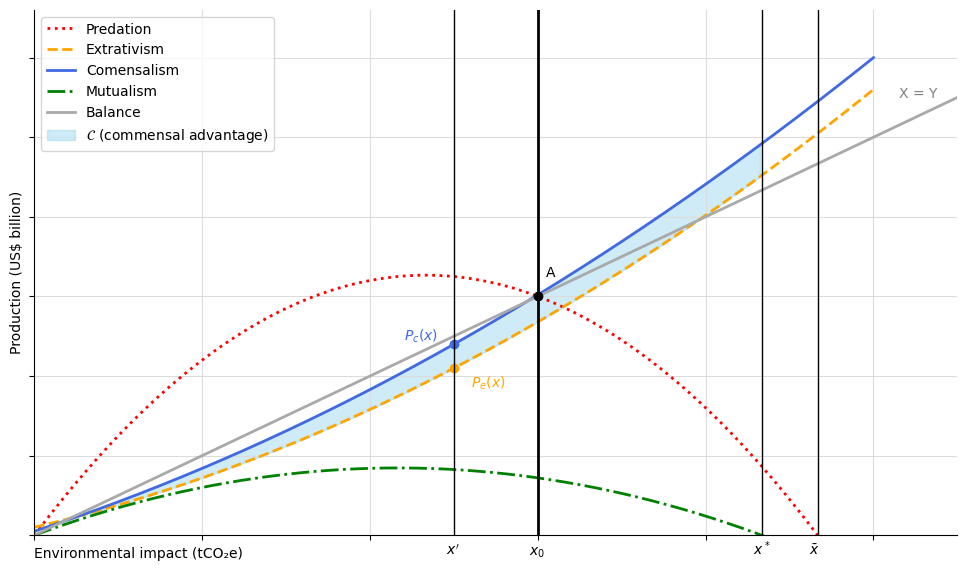
\includegraphics[width=\linewidth]{Figuras/eco_interactions.png}
  \vspace{-0.8em}
  \caption*{\textbf{\small Graph 1 – Theoretical supply curves under different ecological-economic strategies.}}
  \vspace{-0.5em}
  \caption*{\footnotesize Source: Author.}
  \label{graph1}
\end{figure}

Graph 1 compares the four ecological-economic paradigms examined in this research, which will be formally conceptualized in Chapter 1, by plotting production ($Y$, in US\$ billion) against environmental impact ($X$, in tons of CO\textsubscript{2}). The gray diagonal line ($X = Y$) represents a sustainability threshold: points above this line indicate that environmental costs exceed economic returns (ecological inefficiency), while points below suggest that production remains ecologically efficient relative to its footprint.

The \textit{predatory curve} (red, dotted) illustrates this dynamic most dramatically. It rises sharply as natural resources are exploited rapidly, but soon reaches a peak and collapses. This trajectory reflects the classical \textit{tragedy of the commons}: short-term maximization leads to irreversible ecological degradation and long-term economic failure. The critical intersection between the predatory trajectory and the balance line, labeled as point $A$ in the graph, is referred to as the \textit{Predatory Equilibrium Threshold} ($x_0$). It marks the end of the ecological credit zone for unsustainable models and represents the boundary of permissible exploitation under high-impact dynamics.

From the perspective of economic commensalism, the shaded area beneath the predatory curve and above the ecological equilibrium line ($X = Y$), from the origin up to $x_0$, can be interpreted as the total ecological stock that a biome or territory can endure before entering irreversible decline. Beyond this point, the system enters a state of net ecological debt, making even high-output strategies economically and ecologically unjustifiable.

The \textit{extractivist curve} (orange, dashed) attempts to moderate this collapse through legal or institutional constraints. While it temporarily extends the productive lifespan of the system, it eventually surpasses the sustainability threshold, indicating that even regulated extraction becomes ecologically inefficient over time. The model fails to maximize long-term productivity and does not prevent cumulative environmental degradation.

The \textit{mutualist curve} (green, dash-dotted) represents a normative ideal found in many conservation policies. It is modeled here as a concave quadratic function with low elasticity, capturing a regime of cautious use and diminishing marginal returns. It remains entirely below the balance line, reflecting ecological prudence, but reaches only modest productivity levels. Such strategies may preserve ecological integrity but tend to be economically unviable without ongoing subsidies or strong non-market incentives.

In contrast, the \textit{commensalist curve} (blue, solid), central to this research, begins conservatively but eventually surpasses the extractivist model in productivity, while remaining closer to the sustainability threshold throughout. Its long-run advantage lies not in avoiding environmental impact entirely, but in producing greater economic returns per unit of ecological cost. This reflects a strategic use of the environment as a regenerative and intertemporal factor of production, rather than a passive input to be depleted.

In this configuration, the difference between the commensalist and extractivist curves, when calculated separately in the regions above and below the balance line, defines the \textit{commensal advantage}: a net gain in production achieved with proportionally lower ecological burden. Chapter 2 will formally assess whether this differential is provable through dynamic optimization, under uncertainty, learning, and adaptive behavior.

Graph 1 also highlights the conceptual role of the integral $\mathcal{C}$, as well as the analytical relevance of the thresholds $x^*$ (end of economic viability of the mutualist model), $\bar{x}$ (collapse of the predatory model), and $x_0$ (ecological equilibrium breach under predation). These landmarks delimit the theoretical scope within which this research aims to demonstrate that a properly incentivized commensal strategy can outperform extractivist alternatives both economically and ecologically. This framework lays the foundation for the simulations developed in Chapter 2.

Integrating ecological categories such as commensalism, mutualism, and predation into economic reasoning helps to overcome the limitations of the current extractivist paradigm, which treats nature merely as a stock of resources to be exploited. Doing so enables a more refined understanding of how ecological dynamics influence production, resilience, long-term sustainability, and allows us to theorize environmental preservation not as a moral constraint, but as a rational economic strategy.

In this context, commensalism is proposed as a conceptual and analytical lens through which to model the asymmetric relationship between productive agents and the environment. Borrowed from ecology, the term denotes a form of interaction in which one party benefits while the other is neither harmed nor helped, a metaphor that, while symbolic, carries deep analytical weight. It suggests that the economy need not function as a parasite upon nature, but can instead coexist with it in a non-degradative and strategically beneficial manner, provided appropriate institutional and incentive structures are in place. 

% ---
\subsection{Implications}
% ---

This study holds the potential to generate both theoretical and practical implications by bridging economics and ecology through a rational, incentive-based framework. Conceptually, it contributes to rethinking production theory by integrating environmental dynamics as endogenous variables. Practically, it opens new pathways for policy design, business models, and institutional arrangements that align profitability with ecological resilience. In doing so, it creates space for socially inclusive and economically viable opportunities rooted in a more rational and productive use of natural resources.

%...
\subsubsection{Theoretical Contributions}
%...

This research presents an innovative framework for reconciling environmental conservation with economic efficiency. The proposed methodology, combining dynamic modeling, game theory, and econometric validation, offers a structured approach to designing market-compatible conservation policies. While ambitious, the model has the potential to inform both academic discourse and real-world policy applications.

This is evident when comparing the different theoretical understandings, preliminarily explained in the introductory topic, with the proposal of this work, to be verified and matured during the course of the research.

% INÍCIO TABELA 1
\renewcommand{\arraystretch}{1.3}

\begin{table}[H]
\centering
\caption{Comparative perspectives on the environment in economic and ecological theories}
\footnotesize % Tamanho da fonte
\resizebox{\textwidth}{!}{%
\begin{tabularx}{\textwidth}{lXXXXX}
\toprule
\textbf{Element} & \textbf{Classical-Neoclassical Economics} & \textbf{Institutional Economics} & \textbf{Ecology and Philosophy} & \textbf{Green Economy} & \textbf{Economic Commensalism (proposed)} \\
\midrule

\textbf{Land Factor} 
& Fixed production factor with diminishing returns; often absorbed into capital (\(K\)).
& Governed by property rights, access rules, and institutional power.
& Foundational and irreplaceable basis of life and ecological balance.
& Natural capital to be priced and incorporated into accounts.
& Dynamic ecological stock with productive potential and strategic reserve function. \\

\textbf{Environment} 
& Externality to be corrected via taxes or regulation.
& Common good subject to institutional failure  (Tragedy of the Commons). 
& Systemic interdependence. It has only intrinsic value. 
& Complementary asset with economic and ecological value. 
& Endogenous strategic factor; source of productivity and ecological payoff. \\

\textbf{Incentives logic} 
& Driven by prices and utility/profit maximization. 
& Shaped by rules, norms, and transaction costs.
& Ethics, ecological responsibility, and limits of growth.
& Financial and regulatory incentives for sustainability 
& Rational, territory-specific, dynamic incentives promoting cooperation and preservation. \\

\textbf{Time treatment} 
& Intertemporal optimization with fixed discounting.
& Path-dependent institutional evolution over time.
& Quasi-irreversible ecological processes.
& Inter-generational planning and ecological risk management.
& Strategic long-term rationality; preservation as anticipatory production logic. \\

\textbf{Unit of analysis} 
& Rational agent (homo economicus).
& Groups, communities, and institutional arrangements. 
& Ecological systems, species interactions, biotic communities. 
& Population and territory with environmental footprint. 
& Rational agent interacting with environment and others under ecological constraints. \\

\textbf{Normative goal} 
& Allocative efficiency and competitive equilibrium 
& Institutional stability and minimization of governance failures. 
& Balance between society and nature; ecological integrity. 
& Economic, ecological, and social sustainability. 
& Alignment of economic rationality with environmental resilience and collective benefit. \\

\bottomrule
\end{tabularx}}

\vspace{0.1em}
\begin{flushleft}
\footnotesize
\textbf{Source:} Author, based on cited literature.
\end{flushleft}

\end{table}
% FIM TABELA 1

In this regard, it is important to emphasize that, given the motivations, hypotheses and purposes of this work, it is necessary to define that the term commensalism is not presented here as an aesthetic analogy, but aims to establish an institutional model of incentives, with implications for public policies, legal design and game theory. To this end, according to the methodology presented, the issue must be investigated in more depth and the hypotheses tested.

%...
\subsubsection{Practical Contributions}
%...

In practical terms, economic commensalism proposes an institutional shift in how environmental variables are treated within productive systems. Rather than framing preservation as a constraint or as a moral obligation, this approach treats environmental integrity as a productive asset that generates returns when preserved and signals ecological costs when degraded. This reconfiguration creates the basis for measurable ecological accountability, incentive-compatible preservation contracts, and financial innovations rooted in real, localized ecological data.

The comparative evidence across biomes, as shown in Table 2, reveals a critical dissonance between legal requirements and scientific tipping points. In the Amazon, where current legal protections exceed the scientific thresholds, preservation is relatively aligned with ecological resilience. However, in the Cerrado and Pantanal, legal baselines are dangerously below ecological thresholds, exposing these regions to irreversible degradation. A commensalist framework can help recalibrate these legal requirements using biophysical indicators, moving toward a dynamic and territory-specific model that anticipates ecological risk rather than reacting to its consequences.

% INÍCIO TABELA 2
\begin{table}[H]
\centering
\caption{Comparison between Deforestation, Scientific Tipping Points and Legal Requirements by Biome}
\label{tab:biomes_threshold}
\footnotesize
\renewcommand{\arraystretch}{1.3}
\begin{tabularx}{\textwidth}{|l|c|c|c|X|}
\hline
\textbf{Biome} & 
\textbf{\begin{tabular}[c]{@{}c@{}}Cumulative\\ Deforestation (\%)\end{tabular}} & 
\textbf{\begin{tabular}[c]{@{}c@{}}Scientific\\ Tipping Point (\%)\end{tabular}} & 
\textbf{\begin{tabular}[c]{@{}c@{}}Legal\\ Requirement (\%)\end{tabular}} & 
\textbf{Alignment with Science} \\ 
\hline

Amazon & 
\textasciitilde17\% & 
20-25\% & 
80\% & 
High (protection above critical threshold) \\ 
\hline

Cerrado & 
\textasciitilde50\% & 
45-55\% & 
20-35\% & 
Low (legal limit below ecological threshold) \\ 
\hline

Pantanal & 
\textasciitilde25\% & 
30\% (hydrological regime) & 
20\% & 
Very low (risk not considered) \\ 
\hline

\end{tabularx}

\vspace{0.1em}
\begin{flushleft}
\footnotesize
\textbf{Source:} Based on \citeonline{lenton2008tipping}, \citeonline{lovejoy2018amazon}, and \citeonline{IPCC2023}.
\end{flushleft}

\end{table}
% FIM TABELA 2

Carbon markets, currently underutilized or poorly regulated, especially at the subnational level, could be radically improved under a commensal logic. Instead of speculative mechanisms disconnected from ecological performance, local carbon pricing and compensation schemes would be anchored in actual biophysical integrity, incentivizing producers to maximize output within ecological safety zones. Instruments such as REDD+, green bonds, CRAs (Certificates of Agribusiness Receivables), and PRAs (Environmental Regularization Programs) would gain effectiveness by shifting from punitive compliance models to reward-based, performance-linked contracts.

In the case of Mato Grosso, where agricultural frontiers coincide with some of the world's most endangered ecosystems, economic commensalism could unlock a new generation of public policies. These would promote preservation not by imposing restrictions, but by enhancing the profitability of sustainable practices. Producers would be motivated to invest in advanced monitoring technologies (such as IoT-based land tracking, AI-enabled forecasting, or precision machinery), not only for productive efficiency but also for environmental certification, credit access, and territorial premiums. This dual payoff structure, productivity and preservation, would improve investment decisions, reduce long-term risk, and expand financial access for rural producers.

Ultimately, the commensalist framework suggests a paradigm shift: from fragmented environmental policy to integrated territorial governance; from reactive command-and-control instruments to proactive ecological valuation; and from short-term extraction to long-term strategic use of natural capital. These transformations carry not only environmental and economic benefits, but also open a path for inclusive development models that reconcile production with the safeguarding of critical ecosystems.

%...
\subsubsection{Research Opportunities}
%...

The approach introduced in this study represents an attempt to compel a major shift in how environmental variables are interpreted, valued, and integrated into economic systems, particularly in frontier areas such as Mato Grosso, where environmental pressures and productive growth are closely intertwined. By transcending a reactive and extractivist mindset, economic commensalism aims to redefine nature not as a mere limitation, but as a dynamic asset capable of providing economic returns. If this perspective proves viable and theoretically sound, the resulting ontological paradigm change will position ecological preservation as a source of revenue and intrinsic value, transforming forests, ecotones, and other preserved ecosystems into fixed capital and financial assets.

From a practical standpoint, this would imply a new architecture for environmental finance. Instead of viewing producers only through the lens of legal compliance, banks and credit institutions can assess their environmental stock — their preserved hectares — as a tangible component of creditworthiness. This will enable the integration of an environmental score into rural credit models and the structured issuance of green financial instruments such as green bonds, CRAs, and sustainability-linked loans indexed to ecological metrics. Under a commensalist logic, landowners would be incentivized to preserve biomes not by coercion, but because the opportunity cost of deforestation would exceed the long-term returns from maintaining ecosystem integrity, especially if local carbon pricing systems become more transparent and decentralized.

Unlike today’s “green” financial instruments, which often operate under a merely cosmetic logic, rewarding actors for not exceeding minimum thresholds, the commensalist framework invites a transition from compensation to value generation without degradation. It promotes investment in capital and labor (particularly human capital), while reducing pressure on natural assets like land and hydrological cycles. Moreover, if our theoretical proposal proves to be coherent, logically valid, and supported by real evidence that its assumptions work in the factual world, it will curb speculative or exaggerated claims from environmental asset sellers by tying remuneration to verifiable local performance, rather than to opaque offset structures. In doing so, it would enhance both the legitimacy and the efficiency of carbon markets and regulatory mechanisms.

Incidentally, in theoretical terms, the introduction of the concept of economic commensalism reorients economic thought itself: from marginalist models based on scarcity and substitution, to integrated systems where preservation and production are jointly optimized. By treating the environment as an endogenous and flexible input, subject to local thresholds and ecological tipping points, this framework allows for a more rational allocation of resources. It enables public policy to move from rigid command-and-control approaches to adaptive, incentive-compatible strategies that better reflect the diversity of biomes and socio-productive realities. In sum, the research opens new avenues for aligning private rationality with public sustainability goals, not by moral persuasion, but through a new institutional logic grounded in ecological productivity and economic profitability.

% ---
\subsection{Possibly Limitations}
% ---

As an emerging and exploratory framework, our research may encounter theoretical and formalization challenges, especially in aligning ecological concepts with established economic modeling tools. Translating ecological dynamics, such as resilience, tipping points, and asymmetrical dependence, into consistent mathematical and econometric models remains a demanding task that may require iterative refinement.

Empirically, the study may also face constraints related to the availability and reliability of disaggregated environmental data — particularly at the biome and property levels in Mato Grosso. Incomplete or outdated land use information, limited access to verified carbon data, and lack of standardized ecological indicators may restrict the precision of empirical tests. These limitations do not invalidate the research but call for cautious interpretation and future methodological adaptations.

\newpage

% fim %
\clearpage
\thispagestyle{fancy}

%%%===========================================

% ===
\section{Final Remarks}
% ===

This thesis aims to address a foundational limitation in mainstream economic theory: the persistent treatment of the environment as an exogenous constraint, external to the logic of production and disconnected from the behavior of economic agents. By proposing the endogenization of environmental resources into the structure of economic reasoning, the research seeks to integrate ecological boundaries into the decision-making processes of producers, firms, and institutions. It would explore the hypothesis that environmental preservation could become a rational, utility-maximizing strategy when ecological limits are clearly defined and economic incentives are structured accordingly.

The research would begin by investigating the theoretical origins and institutional consequences of treating nature as a non-scarce or marginal input. It would argue that this framing contributes to inefficiencies, externalities, and ecological collapse, especially when resource exploitation exceeds scientifically defined thresholds. Although instruments such as carbon markets, environmental certificates, and payments for ecosystem services already exist, they tend to operate as fragmented compensations or marginal rewards, rather than as central components of the economic system. The thesis would therefore aim to reinterpret these tools through a conceptual framework in which ecological rationality is aligned with economic incentives.

From this perspective, the second part of the thesis would seek to translate the proposed theoretical insights into a coherent structure capable of clarifying how different incentive configurations — whether economic, institutional, or territorial — might shape the behavior of agents facing environmental trade-offs. The core question would not be whether preservation is desirable in normative terms, but whether it could become the most advantageous course of action given the constraints and opportunities defined by the system. This would require situating the environment not as a passive boundary condition, but as an active variable influencing utility, productivity, and long-term resilience.

The final section of the research would aim to test whether the hypotheses outlined in the earlier chapters are supported by empirical patterns and institutional dynamics observed in a real-world context. The state of Mato Grosso — marked by high agricultural output and ecological diversity — would provide a critical setting in which to examine the feasibility of applying such a framework. Ultimately, the thesis would propose that an economy structured around commensal logic could enable the state to act not as a punitive enforcer, but as a catalyst of value — rewarding those who operate in synergy with environmental constraints, and fostering a productive system in which conservation is no longer a cost, but a dominant strategy.

This research introduces an integrated framework where environmental limitations are viewed not as externalities but as internal factors influencing productive decisions, potentially offering both theoretical and practical insights. On a theoretical level, it aims to challenge the prevailing paradigm by altering the principles of production theory, introducing ecological rationality into the agents' utility, and reframing conservation as a strategic option, not a limitation. Practically, it could guide the creation of localized policies and incentives that bolster both environmental resilience and economic success. By doing so, this work may create new possibilities for regional governance, sustainable certification schemes, and data-driven public planning, especially in areas like Mato Grosso where ecological and economic limits intersect. More generally, it proposes a paradigm in which environmental preservation is not in opposition to economic development but is seen as the most logical and beneficial path forward.


\newpage

% fim %

% ==== APENDICES ====
\clearpage
\appendix
\renewcommand{\thesection}{\Alph{section}.}
\thispagestyle{fancy}

%%%===========================================
\section{Timeline}

\subsection{Research Schedule and Timeline}

According to the official academic calendar of the doctoral program, the student’s \textbf{enrollment began on January 25, 2024}, which also marks the starting point for the time count toward graduation requirements. Thus, \textbf{the maximum allowed period for submitting the final dissertation is October 25, 2028}, with the \textbf{deadline for registering for the qualifying examination set for June 1, 2026}. Within this timeframe, the research plan is structured to ensure consistent progress and early completion of key milestones, allowing time for feedback, adjustments, and deepening of the theoretical and empirical components as necessary.

\begin{table}[H]
\centering
\label{tab:timeline}
\renewcommand{\arraystretch}{1.3}
\footnotesize
\begin{tabularx}{\textwidth}{|c|X|}
\hline
\textbf{Period} & \textbf{Milestones and Planned Activities} \\
\hline
\textbf{2nd Semester 2025} & * Start of research activities. * Final refinement of the research design and hypotheses. * Initial literature review and consolidation of the theoretical basis for Chapter 1. * Drafting of the introduction and early theoretical articulation. \\
\hline
\textbf{Year 2026} & * Completion of Chapter 1. * Development of formal theoretical and mathematical models (Chapter 2). * Preparation for the qualifying exam (by June 2026). * Initial design of data structure and econometric strategy. \\
\hline
\textbf{Year 2027} & * Empirical validation and econometric modeling (Chapter 3). * Data collection and processing. * Testing of the Beta Models. * Integration of theoretical and empirical findings. \\
\hline
\textbf{Year 2028 (until Oct)} & * Final editing, adjustments, formatting, and submission of the dissertation. * Preparation for defense. * Optional deepening of case studies or production of related academic papers. \\
\hline
\end{tabularx}
\end{table}

This schedule was designed not only to meet the program's formal deadlines, but also to anticipate potential difficulties in modeling, data access, or empirical validation. The timeline includes deliberate margins to accommodate unforeseen circumstances and provides flexibility for refining the research, deepening promising analytical aspects, and exploring new hypotheses that may emerge throughout the doctoral process.


\newpage

% fim %
\clearpage
\thispagestyle{fancy}

%%%===========================================
\section{On the Use of AI}

\textit{This document employed generative artificial intelligence (AI) tools, including machine learning-based language models, to support writing assistance, idea organization, textual coherence verification and mathematical and logical revision.}
\newline

\noindent\textit{In this sense, it is important to emphasize that AI was used only as an auxiliary tool, with all the curatorial work, critical analysis, theoretical modeling, mathematical formalization, statistical validation and intellectual contributions conceived by the main author of the writing.}

% fim %

% ==== REFERENCIAS ====
\clearpage
\bibliographystyle{abntex2-alf-negrito}
\bibliography{library}

\end{document}
